\documentclass[
  bibliography=totoc,     % Literatur im Inhaltsverzeichnis
  captions=tableheading,  % Tabellenüberschriften
  titlepage=firstiscover, % Titelseite ist Deckblatt
]{scrartcl}

% LaTeX2e korrigieren.
\usepackage{fixltx2e}
% Warnung, falls nochmal kompiliert werden muss
\usepackage[aux]{rerunfilecheck}

% deutsche Spracheinstellungen
\usepackage{polyglossia}
\setmainlanguage{german}

% unverzichtbare Mathe-Befehle
\usepackage{amsmath}
% viele Mathe-Symbole
\usepackage{amssymb}
% Erweiterungen für amsmath
\usepackage{mathtools}

% Fonteinstellungen
\usepackage{fontspec}
\defaultfontfeatures{Ligatures=TeX}

\iffalse
\usepackage[
  math-style=ISO,    % \
  bold-style=ISO,    % |
  sans-style=italic, % | ISO-Standard folgen
  nabla=upright,     % |
  partial=upright,   % /
]{unicode-math}

\setmathfont[range={\mathscr, \mathbfscr}]{XITS Math}
\setmathfont[range=\coloneq]{XITS Math}
\setmathfont[range=\propto]{XITS Math}
\fi

% make bar horizontal, use \hslash for slashed h
\let\hbar\relax
\DeclareMathSymbol{\hbar}{\mathord}{AMSb}{"7E}
\DeclareMathSymbol{ℏ}{\mathord}{AMSb}{"7E}



% richtige Anführungszeichen
\usepackage[autostyle]{csquotes}

% Zahlen und Einheiten
\usepackage[
  locale=DE,                   % deutsche Einstellungen
  separate-uncertainty=true,   % Immer Fehler mit \pm
  per-mode=symbol-or-fraction, % m/s im Text, sonst Brüche
]{siunitx}

% chemische Formeln
\usepackage[version=3]{mhchem}

% schöne Brüche im Text
\usepackage{xfrac}

% Floats innerhalb einer Section halten
\usepackage[section, below]{placeins}
% Captions schöner machen.
\usepackage[
  labelfont=bf,        % Tabelle x: Abbildung y: ist jetzt fett
  font=small,          % Schrift etwas kleiner als Dokument
  width=0.9\textwidth, % maximale Breite einer Caption schmaler
format=plain
]{caption}
% subfigure, subtable, subref
\usepackage{subcaption}

% Grafiken können eingebunden werden
\usepackage{graphicx}
% größere Variation von Dateinamen möglich
\usepackage{grffile}
\usepackage{pdfpages}

% Standardplatzierung für Floats einstellen
\usepackage{float}
\floatplacement{figure}{htbp}
\floatplacement{table}{htbp}

% schöne Tabellen
\usepackage{booktabs}
\usepackage{multirow}

%griechische Buchstaben aufrecht
\usepackage{upgreek}

% Seite drehen für breite Tabellen
\usepackage{pdflscape}

% Literaturverzeichnis
\usepackage{biblatex}
% Quellendatenbank
\addbibresource{lit.bib}
\addbibresource{programme.bib}

%Keine Leertaste hinter Kommata
\usepackage{ziffer}



% Hyperlinks im Dokument
\usepackage[
  unicode,
  pdfusetitle,    % Titel, Autoren und Datum als PDF-Attribute
  pdfcreator={},  % PDF-Attribute säubern
  pdfproducer={}, % "
]{hyperref}
% erweiterte Bookmarks im PDF
\usepackage{bookmark}
% Trennung von Wörtern mit Strichen
\usepackage[shortcuts]{extdash}
%neue befehle
\def\d{\text{d}}
%für wrapfigure:
\usepackage{graphicx}
\usepackage{wrapfig}

\author{
  Kevin Schmidt%
  \texorpdfstring{
    \\
    \href{mailto:kevin3.schmidt@tu-dortmund.de}{kevin3.schmidt@tu-dortmund.de}
  }{}%
  \texorpdfstring{\and}{, }
  Simone Mender
  \texorpdfstring{
    \\
    \href{mailto:simone.mender@tu-dortmund.de}{simone.mender@tu-dortmund.de}
  }{}
}
\publishers{TU Dortmund – Fakultät Physik}


%%% Hier definiert man Titel, Autor und Datum %%%%%%%%%%%%%%%%%%%%%%%%%%%%%%%%%

\subject{Versuch 41}
\title{Debye-Scherrer-Aufnahmen}
\date{
  Durchführung: 31.10.2016
  \hspace{3em}
  1. Abgabe: xx.11.2016
}

%%%%%%%%%%%%%%%%%%%%%%%%%%%%%%%%%%%%%%%%%%%%%%%%%%%%%%%%%%%%%%%%%%%%%%%%%%%%%%%

\begin{document}

\maketitle
\thispagestyle{empty}
\tableofcontents
\newpage

%\section{Zielsetzung}

%\section{Zielsetzung}
Durch das Debye-Scherrer-Verfahren soll die Kristallstruktur zweier Proben bestimmt werden...
\textcolor{red}{...}
\section{Theorie}
Mit dem Debye-Scherrer-Verfahren sollen Kristallstrkturen untersucht werden.
Daher wird zunächst allgemein auf die theoretische Beschreibung von Kristallstrukturen eingegangen.
Zudem wird in diesem Kapitel die Beugung von Röntgenstrahlen an Kristallen und weitere theroretische Grundlagen zum Debye-Scherrer-Verfahren erläutert.

\subsection{Beschreibung von Kristallstrukturen}
Eine Kristallstuktur lässt sich durch ein Punktgitter beschreiben.
Ein einzelner Gitterpunkt besteht aus einem einzelnen Atom oder einer Atomgruppe.
Dieses Atom oder diese Atomgruppe wird als Basis bezeichnet.
Das Gitter beschreibt die periodische Anordnung der Atome im Kristall.
Diese Anordnung lässt sich durch die Basisvektoren $\vec a_i$ ($i=1,2,3$) beschreiben.
Durch Linearkombinationen dieser Vektoren lässt sich jeder Gitterpunkt von einer beliebigen Basis aus erreichen.\\
Das von den Vektoren aufgespannte Volumen heißt Elementarzelle.
Befindet sich in dieser Elementarzelle nur ein Gitterpunkt ist die Elementarzelle primitiv.
Betrachtet man nur die Symmetrieeigenschaften der Kristallstrukturen gibt es 14 unterschiedliche Gittertypen, die Bravais-Gitter genannt werden.\\
Im folgenden Unterkapitel \ref{sec:kubisch} wird genauer auf die kubischen Kristallstrukturen eingegangen.
Zudem wird im Unterkapitel \ref{sec:miller} auf die Kennzeichnung von Netzebenen durch Millersche Indizes sowie auf die Berechnung von Abständen zwischen den Netzebenen eingegangen.
%Da mithilfe von Beugung von Röntgenstrahlen an Kristallgittern auf die Struktur dieser Kristallgitter rückgeschlossen werden kann, wird im Unterkapitel \ref{sec:Beugung} auf die theoretische Beschreibung dieser Methode eingangen.

\subsubsection{Kubische Kristallstukturen}
\label{sec:kubisch}
Das kubische Kristallgitter ist das Bravais Gitter, welches in der Natur am häufigsten vorkommt.
Das kubisch-primitive Gitter besteht aus einer Würfelstruktur, wobei sich an jedem Eckpunkt des Würfels ein Gitterpunkt befindet.
Enthält die Gitterzelle  zusätzlich einen Gitterpunkt zentriert in der Mitte des Würfels, heißt die Gitterstruktur kubisch-raumzentriert.
Wenn sich stattdessen neben den Eckatomen jeweils ein zusätzlicher Giterpunkt in der Mitte jede Würfelfläche befindet, wird die Struktur kubisch-flächenzentriert genannt.\\
Einige wichtige Kristalltrukturen, wie beispielsweise die Dimant- oder die Flourid\-/Struktur, setzten sich aus kubisch-flächenzentrierten Strukturen zusammen.
\textcolor{red}{noch was ergänzen?}

\subsubsection{Gitterebenen}
\label{sec:miller}
Als Gitterebene wird eine Ebene bezeichnet die durch die Gitterpunkte des Kristallstruktur aufgespannt wird.
Aufgrund der Symmetrie des Kristalls gehört zu jeder Netzebene eine Netzebenenscharr.
Alle Netzebenen einer Netzebenenscharr sind parallel zueinander und äquidistant.
Die Lage einer Netzebenenscharr im Raum wird durch die Millerschen Indizes $(hkl)$ festgelegt.
Für die Berechnung der Millerschen Indizes wird das Reziproke der Achsenabschitte der entsprechenden Ebene mit einem beliebigen Faktor ganzzahlig gemacht.
Zwischen zweier benachbarten Netzebenen der gleichen Netzebenenscharr befindet sich der Abstand
\begin{equation}
  d=\frac{a}{\sqrt{h^2+k^2+l^2}},
\end{equation}
wobei $a$ der Betrag der Basisvektoren ist.

\subsection{Beugung von Röntgenstrahlen an Kristallen}
\label{sec:Beugung}
Mit Röntgenstrahlung bezeichnet man elektromagnetische Wellen mit Energien zwischen $\SI{5}{\kilo\electronvolt}$
und einigen hundert \si{\kilo\electronvolt}.
Die Wechselwirkung von Röntgenstrahlung mit den Atomen eines Kristalls kann durch einen klassischen Streuprozess beschrieben werden.
Da sowohl die Elektronen als auch die Atomkerne der Gitteratome durch das elektrische Wechselfeld  angeregt werden, beginnen sie selbst zu schwingen und elektrische Strahlung zu emittieren.
Da sich die Gitteratome in einer räumlichen Symmertrie zueinander befinden, kann diese emittierte Strahlung miteinander interferieren.
Damit die Streuwinkel gut messbar sind, sollte sich die Wellenlänge der Röntgenstrahlung in der Größenordnung \si{\angstrom} befinden.\\
Die von der Röngenstrahlung angeregten Teilchen können als Hertzscher Dipol aufgefasst werden.
Daher beträgt die Intensität der emittierten Strahlung
\begin{equation}
  \label{eq:5}
I_\text{e}(r,\theta)=I_0\left(\frac{\mu_0 q^2}{4\pi m}\right)^2\frac{1+\cos^2(2\theta)}{2r^2}.
\end{equation}
Dabei ist $I_0$ die Intensität des einfallenden Strahles, $r$ die Distanz zum Dipol, $\mu_0$  die magnetische Feldkonstante\footnote{$\mu_0=\SI{1,2566e-6}{\newton\per\square\ampere}$}, $2\theta$ der Winkel zwischen einfallendem und gestreutem Strahl, $q$ die Ladung und $m$ die Masse des schwingenden Teilchens.
Da die Intensität antiprotional zur Masse des schwingenden Teilchens ist, ist die Emission der Atomkerne vernachlässigbar gegenüber der Emission der Elektronen.
Da die Ausdehnung der Elektronenhülle aufgrund der überharten Röntgenstrahlung nicht vernachlässigbar ist, kommt es zu einem Phasenunterschied $\Delta \varphi$ zwischen den Intensitäten der Strahlung durch die einzelnen Elektronen.
Durch diesen Phasenunterschied unterscheidet sich die  Streuintensität $I_\text{a}$ eines Atoms mit der Kernladungszahl $z$ von der über die Formel \ref{eq:5} berechneten Streuintensität $I_\text{e}$.
Das Verhältnis
\begin{equation}
  \frac{I_\text{a}}{I_\text{e}}=f^2
\end{equation}
dieser Intensitäten ist gleich dem Quadrat des Formfaktors $f$. Dieser Faktor berechnet sich durch die Fourier-Transformation der Ladungsverteilung $\rho(\vec r)$ der Elektronen:
\begin{equation}
  f=\int_\text{Hülle}\exp\left(i\Delta\varphi\right)\rho(\vec r)\,\d^3r.
\end{equation}
\begin{wrapfigure}{r}{0.4\textwidth}
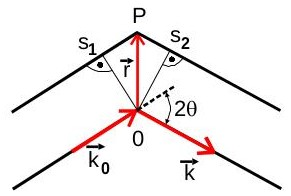
\includegraphics[width=0.4\textwidth]{abb8.jpg}
\caption{Geometrische Überlegung zur Berechnung des Phasenunterschiedes $\Delta \varphi$ zweier Wellen die an den Punkten O und P gestreut werden. Abbildung entnommen aus \cite{V41}.}
\label{abb:8}
\end{wrapfigure}
Durch geometrische Überlegungen, welche in Abbildung \ref{abb:8} dargestellt sind, wird deutlich, dass der Phasenunterschied
\begin{equation}
  \label{eq:7}
  \Delta \varphi=2\pi \frac{\Delta s}{\lambda}=2\pi \frac{s_1+s_2}{\lambda}=2\pi\vec r \cdot \left(\vec k- \vec k_0\right)
\end{equation}
beträgt.
Um nun die Streuung am Kristallgitter zu beschreiben, muss  der Phasenunterschied zwischen zwei Wellen, die an unterschiednlichen Atomen in der Elementarzelle gestreut werden, bekannt sein.
Wenn das eine Atom sich im Ursprung des Koordinatensystems befindet und sich der Platz des anderen Atoms durch den Ortsvektor $\vec r_j$ beschreiben lässt, beträgt diese Phasendifferenz
\begin{equation}
  \Delta \varphi_j = 2\pi \vec r_j\cdot \left(\vec k-\vec k_0\right).
\end{equation}
Die gesamte Streuamplitude $A$ berechnet sich durch die Summe aller einzelnen Intensitäten:
\begin{equation}
  A=\sum_jf_j\exp\left(-2\pi i \vec r _j\cdot\left(\vec k-\vec k_0\right)\right)I_\text{e},
\end{equation}
wobei $f_j$ der Formfaktor des entsprechendes Atoms ist.
Stellt man nun die Ortsvektoren durch die Basisvektoren $\vec a_i$ dar, erhält man die Strukturamplitude
\begin{equation}
  S=\sum_jf_j\exp\left(-2\pi i \left(x_j\vec a_1+x_j\vec a_2+x_j\vec a_3 \right)\cdot\left(\vec k-\vec k_0\right)\right)I_\text{e}.
\end{equation}
Dabei gilt für die Beträge der Basisvektoren $|\vec a_i|\le 1$.
Das Betragsquadrat der Strukturamplitude  $|S^2|=SS^*$ heißt Strukturfaktor und gibt das Verhältnis von einer Elementarzelle und von einem einzelnen Elektron gestreuten Intensitäten an.
Um Streuung an Elementarzellen, die in einem periodischen Gitter angeordnet sind, zu betrachten, wird eine Elementarzelle als punktförmig angenommen, sodass die Bragg-Bedingung
\begin{equation}
  n\lambda=2d\sin\left(\theta\right)~~~\text{mit}~n=1,2,...
\end{equation}
gilt.
Diese Bragg-Bedingung kann auch durch die Wellenzahlvektoren und den reziproke Gittervektor $\vec G$ dargestellt werden:
\begin{equation}
  \vec k -\vec k_0 =\vec G.
\end{equation}
Der reziproke Gittervektor
\begin{equation}
  \vec G= h g_1+kg_2+lg_3
\end{equation}
besteht aus den Millerschen Inzides $hkl$ und den Basisvektoren
\begin{equation}
   \vec g_1=\frac{\vec a_2\times \vec a_3}{\vec a_1 \cdot \left(\vec a_2 \times \vec a_3\right)}, ~~  \vec g_2=\frac{\vec a_3\times \vec a_1}{\vec a_1 \cdot \left(\vec a_2 \times \vec a_3\right)}~~\text{und}~~  \vec g_3=\frac{\vec a_1\times \vec a_2}{\vec a_1 \cdot \left(\vec a_2 \times \vec a_3\right)}
\end{equation}
des reziproken Gitters.
Die Strukturamplitude
\begin{equation}
  S(h,k,l)=\sum _j f_j\exp\left(x_j h+ y_jk+z_j l\right)
\end{equation}
berechnet sich nun in Abhängigkeit von den Millerschen Indizes und der Orte der Atome $\vec r_j=\left(x_j, y_j, z_j\right)^\text{T}$  in der Elementarzelle.

%\input{aufbau.tex}
\section{Durchführung und Versuchsaufbau}

Damit die Kristallstruktur der zu untersuchenden Probe bestimmt werden kann, soll diese mit Röntgenstrahlung bestrahlt werden.
Es ist zu beachten, dass vor Beginn der Messung die Probe richtig präperiert wird. Dazu wird diese mit Hilfe eines Mörsers zerkleinert und anschließend auf einen vorgefetteten
Zylinder angebracht.
Dadurch sind die Ausrichtungen der Kristalline statistisch verteilt und es ist gewährleistet, dass Bragg-Reflexe in allen Richtungen auftreten.
Anschließend kann die Probe im Versuchsaufbau, einem Kameragehäuse, platziert werden. Ein Elektromotor dreht die Probe während der Messung, damit auch bei grobkörnigen
Probenmaterial die Kristalline verteilt sind.\newline
Die Bragg-Reflexe sollen mit Hilfe eines Fotofilms detektiert werden. Aus diesem Grund wird ein Filmstreifen ringförmig an der Innenseite des Kameragehäuses
befestigt. Der Filmstreifen besitzt zwei Öffnungen für den
Röntgenstrahl. Diese Öffnungen liegen so, dass sie die $180\,\text{°}$ Ebene makieren\newline.
Die Röntgenstrahlung wird durch eine Kupferanode erzeugt. Wenn diese auf die Probe trifft, wird sie mit dem Öffnungswinkel $2\theta$ gestreut. Das Beugungsmuster kann
anschließend auf dem Filmstreifen sichtbar gemacht werden.
Eine Darstellung des Versuchsaufbaus ist in Abbildung \ref{abb:aufbau} dargestellt.\newline
Die Messung wird für zwei verschiedene Proben durchgeführt. Um die Bragg-Reflexionen auf dem Film möglichst genau auswerten zu können, wird die Metall-Probe
$2\,\text{Stunden}$ und die Salz-Probe $3\,\text{Stunden}$ lang bestrahlt.

\begin{figure}
  \centering
  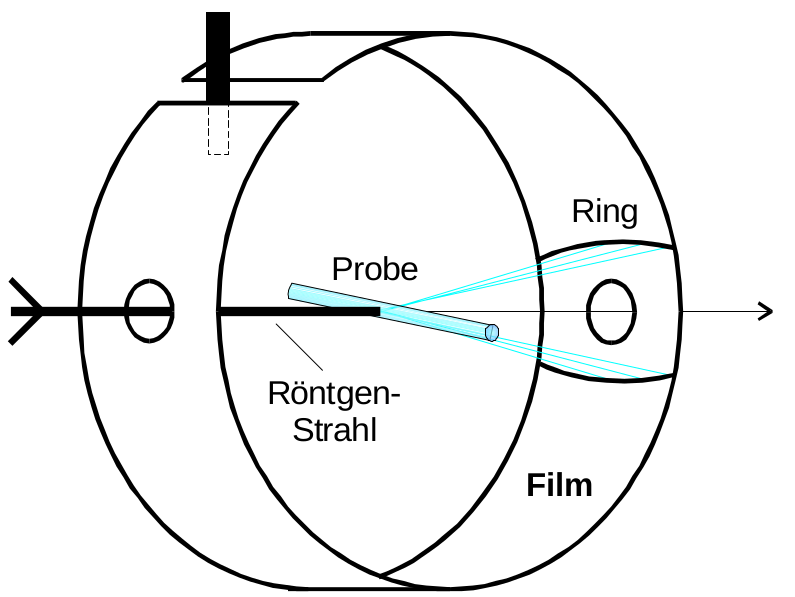
\includegraphics[scale=0.35]{aufbau.png}
  \caption{Versuchsaufbau zur Kristallstrukturbestimmung mit Hilfe des Debye-Scherrer-Verfahrens. In der Abbildung wird die Filmmethode dargestellt. Die Röntgenstrahlen werden an der zylindrischen
  Probe gebeugt. Das Beugungsmuster kann anschließend auf dem Filmstreifen sichtbar gemacht werden. Abbildung entnommen aus \cite{V41}.}
  \label{abb:aufbau}
\end{figure}

%\input{vorbereitung.tex}
%\section{Auswertung}

Zur Auswertung der Messdaten werden die üblichen Formeln für den Mittelwert und die Standardabweichung verwendet. Die Fehlerrechnung wird mittels
Gaußscher Fehlerfortpflanzung durchgeführt. Zusätzlich werden Python 3.5.2 für die Berechnungen, matplotlib.pyplot zum Erstellen der Graphen und
scipy.odr zur Durchführung der lineare Ausgleichsrechnung benutzt.

\subsection{Bestimmung der Gitterstruktur mit Hilfe der Braggreflexe}



Der entwickelte Film enthält kreiförmige Braggreflexe, die charakteristisch für die jeweillige Probe sind. Anhand der Reflexe kann auf die Gitterstruktur der
Probe geschlossen werden und somit die Gitterkonstante bestimmt werden.
Als Referenzwerte werden die Miller'schen Indizes in Gleichung \eqref{eq:streuamplitude} variert und die Reflexe ermittelt, für die die Streuamplitude nicht verschwindet.
Die Ergebnisse für
verschiedene Gitterstrukturen sind in Tabelle \ref{tab:referenz} dargestellt.\newline
Nun sollen die Reflexe auf dem Film mit den Referenzwerten in der Tabelle verglichen werden. Dafür wird der Abstand der Reflexe vom Eintrittsloch der Kamera bestimmt. Ein
Vorteil dabei besteht darin, dass die Kamera einen Umfang von genau $\SI{360}{\milli\meter}$ besitzt. Somit können die Abstände direkt als Winkel
$2\theta$ abgelesen werden. Mit Hilfe der Braggbedingung \eqref{eq:bragg} und der Wellenlänge der Röntgenstrahlung von
$\lambda = \SI{1,54286}{\angstrom}$, welche sich aus dem Mittelwert der $K_\alpha$- und der

\begin{table}[H]
  \centering
  \begin{subtable}{.49\textwidth}
      \centering
      \begin{tabular}{
          S[table-format=3.0]
          S[table-format=2.0]
          S[table-format=1.3]}
          \toprule
          $\text{hkl}$ & $\text{N}$ & $\sqrt[]{N_\text{i}\, / \, N_1}$ \\ \midrule
          100 & 1   & 1,000 \\
          110 & 2   & 1,414 \\
          111 & 3   & 1,732 \\
          200 & 4   & 2,000 \\
          210 & 5   & 2,236 \\
          211 & 6   & 2,449 \\
          220 & 8   & 2,828 \\
          221 & 9   & 3,000 \\
          300 & 9   & 3,000 \\
          310 & 10  & 3,162 \\
          311 & 11  & 3,317 \\
          222 & 12  & 3,464 \\
          320 & 13  & 3,606 \\
          321 & 14  & 3,742 \\
          400 & 16  & 4,000 \\
          \bottomrule
      \end{tabular}
      \caption{sc-Gitterstruktur}
    \end{subtable}
    \begin{subtable}{.49\textwidth}
        \centering
    \begin{tabular}{
        S[table-format=3.0]
        S[table-format=2.0]
        S[table-format=1.3]}
        \toprule
        $\text{hkl}$ & $\text{N}$ & $\sqrt[]{N_\text{i}\, / \, N_1}$ \\ \midrule
        110 & 2   & 1,000 \\
        200 & 4   & 1,414 \\
        211 & 6   & 1,732 \\
        220 & 8   & 2,000 \\
        310 & 10  & 2,236 \\
        222 & 12  & 2,449 \\
        321 & 14  & 2,646 \\
        400 & 16  & 2,828 \\
        330 & 18  & 3,000 \\
        411 & 18  & 3,000 \\
        420 & 20  & 3,162 \\
        332 & 22  & 3,317 \\
        422 & 24  & 3,464 \\
        431 & 26  & 3,606 \\
        510 & 26  & 3,606 \\
        \bottomrule
    \end{tabular}
    \caption{bcc-Gitterstruktur}
  \end{subtable}
  \begin{subtable}{.49\textwidth}
      \centering
        \vspace*{5mm}
      \begin{tabular}{
          S[table-format=3.0]
          S[table-format=2.0]
          S[table-format=1.3]}
          \toprule
          $\text{hkl}$ & $\text{N}$ & $\sqrt[]{N_\text{i}\, / \, N_1}$ \\ \midrule
          111 &  3  & 1,000 \\
          200 &  4  & 1,155 \\
          220 &  8  & 1,633 \\
          311 & 11  & 1,915 \\
          222 & 12  & 2,000 \\
          400 & 16  & 2,309 \\
          331 & 19  & 2,517 \\
          420 & 20  & 2,582 \\
          422 & 24  & 2,828 \\
          333 & 27  & 3,000 \\
          511 & 27  & 3,000 \\
          440 & 32  & 3,266 \\
          531 & 35  & 3,416 \\
          442 & 36  & 3,464 \\
          600 & 36  & 3,464 \\
          \bottomrule
      \end{tabular}
      \caption{fcc-Gitterstruktur}
    \end{subtable}
    \begin{subtable}{.49\textwidth}
      \vspace*{5mm}
        \centering
    \begin{tabular}{
        S[table-format=3.0]
        S[table-format=2.0]
        S[table-format=1.3]}
        \toprule
        $\text{hkl}$ & $\text{N}$ & $\sqrt[]{N_\text{i}\, / \, N_1}$ \\ \midrule
        111 & 3  & 1,000 \\
        220 & 8  & 1,633 \\
        311 & 11 & 1,915 \\
        400 & 16 & 2,309 \\
        331 & 19 & 2,517 \\
        422 & 24 & 2,828 \\
        333 & 27 & 3,000 \\
        511 & 27 & 3,000 \\
        440 & 32 & 3,266 \\
        531 & 35 & 3,416 \\
        620 & 40 & 3,651 \\
        533 & 43 & 3,786 \\
        444 & 48 & 4,000 \\
        551 & 51 & 4,123 \\
        711 & 51 & 4,123 \\
        \bottomrule
    \end{tabular}
    \caption{Diamant-Gitterstruktur}
  \end{subtable}
    \caption{Auftretende Beugungsreflexe bei verschiedenen Gittertypen. Es werden jeweils die Miller'schen Indizes $hkl$, die Summe $N$ der einzelnen Werte $h$, $k$, $l$
    und der Quotient $\sqrt[]{N_\text{i}/N_1}$
    angegeben. Die Tabellen dienen als Referenzwerte, um die Kristallstruktur der Probe zu ermitteln.}
    \label{tab:referenz}
\end{table}


$K_\beta$-Linie ergibt, können die Netzebenenabstände bestimmt werden. Anschließen wird das Verhältnis $d_1 / d_\text{i}$ für die verschiedenen Reflexe gebildet.\newline
Damit die Gitterkonstante der Probe bestimmt werden kann, wird Gleichung \eqref{eq:d} in Gleichung \eqref{eq:bragg} eingesetzt. Es ergibt sich der Ausdruck
\begin{equation}
  \frac{\lambda}{2\sin(\theta)}\,\,\sqrt[]{h^2+k^2+l^2}=d\,\,\sqrt[]{N}=a.
\end{equation}
Durch Normieren dieses Ausdruck kann der Zusammenhang
\begin{equation}
\frac{d_1}{d_\text{i}}=\sqrt[]{N_\text{i}\, / \, N_1}
\end{equation}
aufgestellt werden. Es wird deutlich, dass die gebildeten Verhältnisse $d_1 / d_\text{i}$ mit den Ausdrücken $\sqrt[]{N_\text{i}\, / \, N_1}$ aus Tabelle
\ref{tab:referenz} verglichen werden können. Somit kann die passende Gitterstruktur der Probe ermittelt werden.
Mit bekannter Gitterstruktur kann anschließend die Gitterkonstante der Probe berechnet werden. Es werden aus den einzelnen Messwerten die verschiedenen
Gitterkonstanten ermittelt und anschließend gegen $\cos^2(\theta)$ aufgetragen. Dann wird eine lineare Ausgleichsrechnung durchgeführt, der y-Achsenabschnitt
liefert dabei den Wert für die Gitterkonstante. Bei der linearen Ausgleichsrechnungen werden sowohl die Unsicherheiten auf den x-Werten, als auch die Unsicherheiten auf
den y-Werten berücksichtigt.

\subsection{Ergebnisse für Metall 2}

In Tabelle \ref{tab:metall} sind die Messwerte für die Probe Metall 2 zu sehen. Zusätzlich sind die berechneten Winkel, die berechneten Gitterabstände und die
daraus resultierenden Verhältnisse $d_1 / d_\text{i}$ zu erkennen.\newline
Ein Vergleich von $d_1 / d_\text{i}$ mit $\sqrt[]{N_\text{i}\, / \, N_1}$ zeigt, dass es sich bei der Probe um eine fcc-Gitterstruktur handelt. Der $222$ Reflex und
der $420$ Reflex konnte jedoch auf dem Film nicht wiedergefunden werden, da diese zu schwach sind.
Somit werden die
N-Werte für die fcc-Gitterstruktur zur Berechnung der Gitterkonstanten verwendet. Die Werte für die Gitterkonstanten sind in der letzten Spalte von
Tabelle \ref{tab:metall} zu finden. In Abbildung \ref{abb:metall} sind die einzelnen Gitterkonstanten gegen $\cos^2(\theta)$ aufgetragen. Die lineare Ausgleichsrechnung liefert
die Parameter
\begin{align*}
  m &= \,\,\,0,1\pm0,1~~~~~\text{und}\\
  a &= 4,73\pm0,02
\end{align*}
Der Wert $a = 4,73\pm0,02$ für den y-Achsenabschnitt entspricht der Gitterkonstante der Probe.


\begin{table}[H]
  \centering
\begin{tabular}{
  S[table-format=2.1(1)]
  S[table-format=2.2(2)]
  S[table-format=1.2(2)]
  S[table-format=1.3(3)]
  S[table-format=1.3]
  S[table-format=2]
  S[table-format=1.2(2)]}
  \toprule
  $\text{r / mm}$ & $\theta\text{ / } ^\circ$ &$\text{d / }\si{\angstrom}$&{$d_1 / d_i\,\,/\,\, \si{\angstrom}$} & $\sqrt[]{N_\text{i}\, / \, N_1}_\text{fcc}$& $\text{N}$  &  $\text{a / }\si{\angstrom}$  \\ \midrule
  33    \pm  1,0    &     16,5 \pm 0,5  &  2,72 \pm 0,08  &    1,00 \pm 0,00     &   1,000 &  3   &    4,70 \pm 0,14       \\
  42    \pm  1,0    &     21,0 \pm 0,5  &  2,15 \pm 0,05  &    1,26 \pm 0,05     &   1,155 &  4   &    4,31 \pm 0,10       \\
  54    \pm  1,0    &     27,0 \pm 0,5  &  1,70 \pm 0,03  &    1,60 \pm 0,05     &   1,633 &  8   &    4,81 \pm 0,08       \\
  61	  \pm  1,0    &     30,5 \pm 0,5  &  1,52 \pm 0,02  &    1,79 \pm 0,06     &   1,915 &  11  &    5,04 \pm 0,07       \\
  76    \pm  1,0    &     38,0 \pm 0,5  &  1,25 \pm 0,01  &    2,17 \pm 0,07     &   2,309 &  16  &    5,01 \pm 0,06       \\
  89    \pm  1,0    &     44,5 \pm 0,5  &  1,10 \pm 0,01  &    2,47 \pm 0,08     &   2,517 &  19  &    4,80 \pm 0,04       \\
  102.5 \pm  1,0    &     51,3 \pm 0,5  &  0,99 \pm 0,01  &    2,75 \pm 0,08     &   2,828 &  24  &    4,84 \pm 0,03       \\
  116   \pm  1,0    &     58,0 \pm 0,5  &  0,91 \pm 0,01  &    2,99 \pm 0,09     &   3,000 &  27  &    4,73 \pm 0,03       \\
  132   \pm  1,0    &     66,0 \pm 0,5  &  0,84 \pm 0,01  &    3,22 \pm 0,10     &   3,266 &  32  &    4,78 \pm 0,02       \\
  148   \pm  1,0    &     74,0 \pm 0,5  &  0,80 \pm 0,01  &    3,38 \pm 0,10     &   3,416 &  35  &    4,75 \pm 0,01       \\
  155   \pm  1,0    &     77,5 \pm 0,5  &  0,79 \pm 0,01  &    3,44 \pm 0,10     &   3,464 &  36  &    4,74 \pm 0,01       \\
  \bottomrule
\end{tabular}
\caption{Messwerte und Ergebnisse für die Probe Metall 2. Es sind die Abstände der Braggreflexe, die Winkel $\theta$, die Netzebenenabstände $d$, sowie die Verhältnisse
$d_1 / d_\text{i}$ angegeben. Zusätzlich sind die Werte für $\sqrt[]{N_\text{i}\, / \, N_1}_\text{fcc}$ mit dem passenden $N$ aufgelistet, damit die Gitterstruktur erkennbar wird.
In der letzten Spalte befinden sich die jeweiligen Werte für die Gitterkonstante $a$.}
\label{tab:metall}
\end{table}


\begin{figure}[H]
  \centering
  \includegraphics[scale=0.45]{probe1.pdf}
  \caption{In der Abbildung sind die Gitterkonstanten $a$ gegen $\cos^2(\theta)$ für die Probe Metall 2 aufgetragen. Zusätzlich ist die mit der Ausgleichsrechnung
  ermittelte Gerade zu erkennen.}
  \label{abb:metall}
\end{figure}

\subsection{Ergebnisse für Salz 2}

In Tabelle \ref{tab:salz} sind die Messwerte für die Probe Salz 2 zu sehen. Zusätzlich sind die berechneten Winkel, die berechneten Gitterabstände und die
daraus resultierenden Verhältnisse $d_1 / d_\text{i}$ zu erkennen.
\begin{table}[H]
  \centering
\begin{tabular}{
  S[table-format=2.1(1)]
  S[table-format=2.1(1)]
  S[table-format=1.2(2)]
  S[table-format=1.2(2)]
  S[table-format=1.3]
  S[table-format=2]
  S[table-format=1.2(2)]}
  \toprule
  $\text{r / mm}$ & $\theta\text{ / } ^\circ$ &$\text{d / }\si{\angstrom}$ &{$d_1 / d_i\,\,\text{/}\,\, \si{\angstrom}$} & $\sqrt[]{N_\text{i}\, / \, N_1}_\text{bcc}$& $\text{N}$  &  $\text{a / }\si{\angstrom}$  \\ \midrule
  32    \pm  1,0    &     16,0 \pm 0,5  &  2,80 \pm 0,09  &    1,00 \pm 0,00     &   1,000 &  2   &    4,00 \pm 0,10       \\
  46,5  \pm  1,0    &     23,3 \pm 0,5  &  1,95 \pm 0,04  &    1,43 \pm 0,05     &   1,414 &  4   &    3,91 \pm 0,08       \\
  56    \pm  1,0    &     28,0 \pm 0,5  &  1,64 \pm 0,03  &    1,70 \pm 0,06     &   1,732 &  6   &    4,02 \pm 0,07       \\
  66	  \pm  1,0    &     33,0 \pm 0,5  &  1,42 \pm 0,02  &    1,98 \pm 0,07     &   2,000 &  8   &    4,01 \pm 0,05       \\
  74    \pm  1,0    &     37,0 \pm 0,5  &  1,28 \pm 0,01  &    2,18 \pm 0,07     &   2,236 &  10  &    4,05 \pm 0,05       \\
  79    \pm  1,0    &     39,5 \pm 0,5  &  1,21 \pm 0,01  &    2,31 \pm 0,07     &   2,449 &  12  &    4,20 \pm 0,04       \\
  89    \pm  1,0    &     44,5 \pm 0,5  &  1,10 \pm 0,01  &    2,54 \pm 0,08     &   2,646 &  14  &    4,12 \pm 0,04       \\
  105   \pm  1,0    &     52,5 \pm 0,5  &  0,97 \pm 0,01  &    2,88 \pm 0,09     &   2,828 &  16  &    3,89 \pm 0,03       \\
  113   \pm  1,0    &     56,5 \pm 0,5  &  0,93 \pm 0,01  &    3,03 \pm 0,09     &   3,000 &  18  &    3,92 \pm 0,02       \\
  117   \pm  1,0    &     58,5 \pm 0,5  &  0,90 \pm 0,01  &    3,10 \pm 0,10     &   3,162 &  20  &    4,05 \pm 0,02       \\
  121   \pm  1,0    &     60,5 \pm 0,5  &  0,89 \pm 0,01  &    3,20 \pm 0,10     &   3,317 &  22  &    4,16 \pm 0,02       \\
  132   \pm  1,0    &     66,0 \pm 0,5  &  0,84 \pm 0,01  &    3,30 \pm 0,10     &   3,464 &  24  &    4,14 \pm 0,02       \\
  143   \pm  1,0    &     71,5 \pm 0,5  &  0,81 \pm 0,01  &    3,44 \pm 0,11     &   3,606 &  26  &    4,15 \pm 0,01       \\
  \bottomrule
\end{tabular}
\caption{Messwerte und Ergebnisse für die Probe Salz 2. Es sind die Abstände der Braggreflexe, die Winkel $\theta$, die Netzebenenabstände $d$, sowie die Verhältnisse
$d_1 / d_\text{i}$ angegeben. Zusätzlich sind die Werte für $\sqrt[]{N_\text{i}\, / \, N_1}_\text{bcc}$ mit dem passenden $N$ aufgelistet, damit die Gitterstruktur erkennbar wird.
In der letzten Spalte befinden sich die jeweiligen Werte für die Gitterkonstante $a$.}
\label{tab:salz}
\end{table}


Ein Vergleich von $d_1 / d_\text{i}$ mit $\sqrt[]{N_\text{i}\, / \, N_1}$ zeigt, dass es sich bei der Probe um eine bcc-Gitterstruktur handelt.
Somit werden die
Referenzwerte für die bcc-Gitterstruktur zur Berechnung der Gitterkonstanten verwendet. Die Werte für die Gitterkonstanten sind in der letzten Spalte von
Tabelle \ref{tab:salz} zu finden. In Abbildung \ref{abb:salz} sind die einzelnen Gitterkonstanten gegen $\cos^2(\theta)$ aufgetragen. Die lineare Ausgleichsrechnung liefert
die Parameter
\begin{align*}
  m &= -0,3\pm0,1~~~~~\text{und}\\
  a &= \,\,4,15\pm0,04
\end{align*}
Der Wert $a = 4,15\pm0,04$ für den y-Achsenabschnitt entspricht der Gitterkonstante der Probe.

\begin{figure}[H]
  \centering
  \includegraphics[scale=0.45]{probe2.pdf}
  \caption{In der Abbildung sind die Gitterkonstanten $a$ gegen $\cos^2(\theta)$ für die Probe Salz 2 aufgetragen. Zusätzlich ist die mit der Ausgleichsrechnung
  ermittelte Gerade zu erkennen.}
  \label{abb:salz}
\end{figure}

%\input{auswertung2.tex}
%\section{Diskussion}



\printbibliography

\end{document}
